We desire to select the gain $K$ and the parameter $p$ so that the time-domain specifications will be satisfied.  The settling time should be less than 4.6 seconds and the overshoot should be less than 5\%. 
\begin{center}
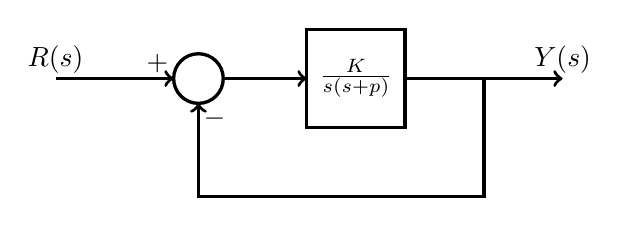
\begin{tikzpicture}[scale=1,inner sep=0pt,outer sep=0pt,very thick,
sysblock/.style={draw,rectangle,inner sep=4pt,minimum width=1.25cm,minimum height=1.25cm,very thick}]

\draw (-2,0) node[draw,circle] (sum1) {$\rule{0pt}{18pt}$};
\draw (0,0) node[sysblock] (G) {$\frac{K}{s(s+p)}$};
\draw[<-] (sum1.180) node[above left=2pt] {$+$} -- ++(-1.5,0) node[above=2pt] {$R(s)$};
\draw[->] (sum1.0) -- (G.180);
\draw[->] (G.0) --  ++(2,0) node[above=2pt] {$Y(s)$};
\draw[->] (G.0) -- ++(1,0) -- ++(0,-1.5) -| (sum1.-90) node[below right=2pt] {$-$};
\end{tikzpicture}
\end{center}
\begin{enumerate}[(a)]
\item Sketch the valid region on the complex plane.
\item Find the values of $K$ and $p$ such that the closed loop exactly meet the condition of 5\% overshoot and a settling time 4.6 seconds.  Mark those points on complex plane also.
\end{enumerate}

